%!TEX ROOT=main.tex
\chapter{Hemodynamické parametry}
Tato kapitola se zaměří na popis hemodynamických parametrů krevního řečiště a na rešerši přístrojů pro měření hemodynamických parametrů krevního řečiště určovaných neinvazivně z tvaru
tlakové křivky.
\section{Krevní tlak}
Krevní tlak je veličina, která vyjadřuje velikost síly proudící krve, působící na stěnu cévy. Velikost krevního tlaku závisí na síle kontrakce srdce, množství krve uvnitř těla,
odporu cév a elasticitě stěny cév. Krevní tlak se uvádí ve dvou typech. Systolický tlak, který vyjadřuje působící sílu krve proti stěně artérie, při kontrakci srdce a diastolický tlak vyjadřuje
tlak, kdy srdce je v klidu mezi jeho činnosti. Krevní tlak se uvádí v jednotkách milimetrů rtuti ($mmHg$), co odpovídá $133.32 \  Pa$. Jako normální lidský krevní tlak se považuje méně jak $120 \ mmHg$ systolického a měně jak  $80 \ mmHg$ diastolického tlaku.
\cite{cite:BP}

\subsection{Centrální aortální tlak}
Centrální aortální tlak je tlak v aortě, do které krev putuje při kontrakci srdce.\cite{cite:CBP}\par
Centrální aortální tlak je možno měřit neinvazivním způsobem, připevněním manžety na horní část ruky nebo zápěstí. Ze snímané tlakové křivky je
možné estimovat centrální aortální tlak.\cite{cite:CBP}

\subsection{Střední arteriální tlak}
Střední arteriální tlak (MAP) je průměrná hodnota krevního tlaku v jednom srdečním cyklu.
\begin{figure}[H]
    \caption{Průběh tlakové křivky pro výpočet středního arteriálního tlaku \cite{cite:4}}
    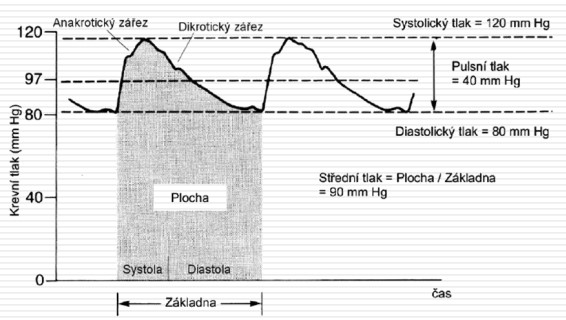
\includegraphics[width=1\textwidth]{pictures/map.jpg}
\end{figure}
Rovnice pro přesný výpočet je
\begin{equation}
    MAP = \frac{1}{T} \int_{t}^{t + T} BP(\tau) d\tau
\end{equation}
Rovnice pro aproximaci je
\begin{equation}
    MAP = DP + \frac{1}{3}(SP - DP)
\end{equation}
Kde $DP$ je diastolický tlak a $SP$ je systolický tlak.
\section{Metody měření krevního tlaku}
Metody měření tlaku můžou být invazivní nebo neinvazivní, manuální čí automatizované. Jedním k nejvíce používaných metod pro neinvazivní měření
krevního tlaku patří auskultační metoda, která používá rtuťového sphygmomanometeru a stetoskopu pro poslouchání krevní vlny. Další nejvíce používaná metoda je oscilometrická metoda.
\cite{cite:Fabian}
\subsection{Oscilometrická metoda}
Oscilometrická metodu měření tlaku využívá navrhovaný systém CarDi. Metoda spočívá v měření objemové pulzace v tepnách přenášející se přes manžetu do přístroje, ve kterém se vyhodnocují.
Amplituda těchto pulzací je závislá na rozdílu tlaku uvnitř a vně tepny, tzv. transmurální tlak. Největší amplituda při je při nulovém transmurální tlaku, to je při hodnotě středního arteriální tlaku.
\cite{cite:Fabian}
\begin{figure}[H]
    \caption{Graf oscilometrických pulzací \cite{cite:Fabian}}
    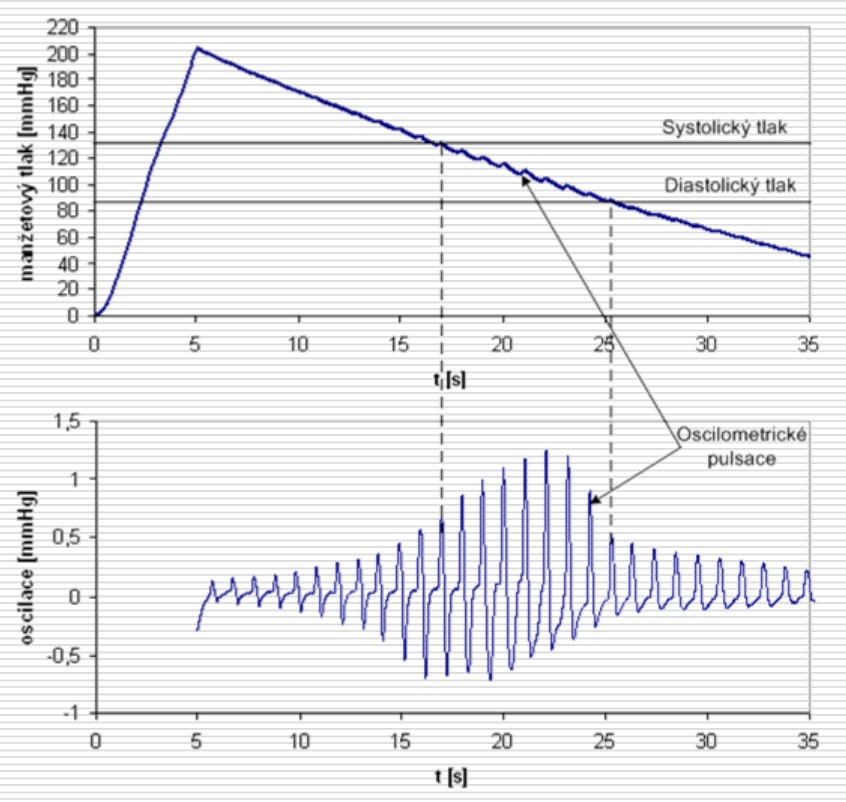
\includegraphics[width=1\textwidth]{pictures/oscilometricky_tlak.jpg}
\end{figure}
\raggedbottom
\section{Rychlost šíření pulzní vlny}
Rychlost šíření pulzní vlny (PWV) je rychlost, během systolické kontrakce srdce, při které tlaková vlna krve se propaguje arteriemi. Parametr PWV je jeden ze základních ukazatelů arteriální
elasticity. Čím je hodnota PWV vetší, tím jsou cévy méně poddajné a výsledkem je zvětšená tuhost artérií.\cite{cite:6}
\begin{figure}[H]
    \caption{Postup odražené krevní tlakové vlny v těle \cite{cite:5}}
    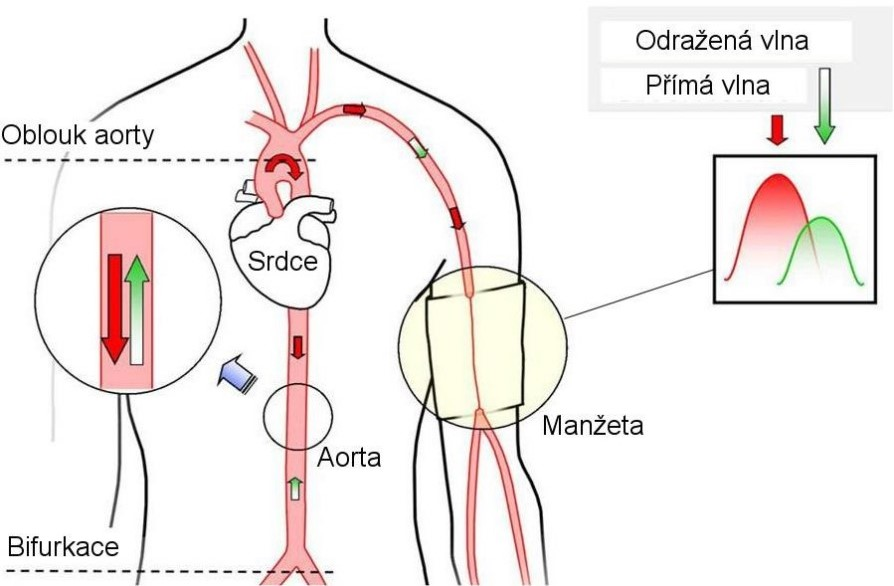
\includegraphics[width=1\textwidth]{pictures/pwv_body.jpg}
\end{figure}
Jeden ze způsobů určení parametru PWV je poměr dvojnásobné vzdálenosti od hrudního zářezu ke stydké kosti $l$ a rozdíl času primární tlakové vlny $t_1$ a odražené tlakové vlny $t_2$.
\begin{equation} \label{eq:pwv}
    PWV = \frac{2l}{t_2 - t_1}
\end{equation}
\begin{figure}[H]
    \caption{Krevní tlaková vlna s vyznačenými parametry pro výpočet parametru PWV. \cite{cite:7}}
    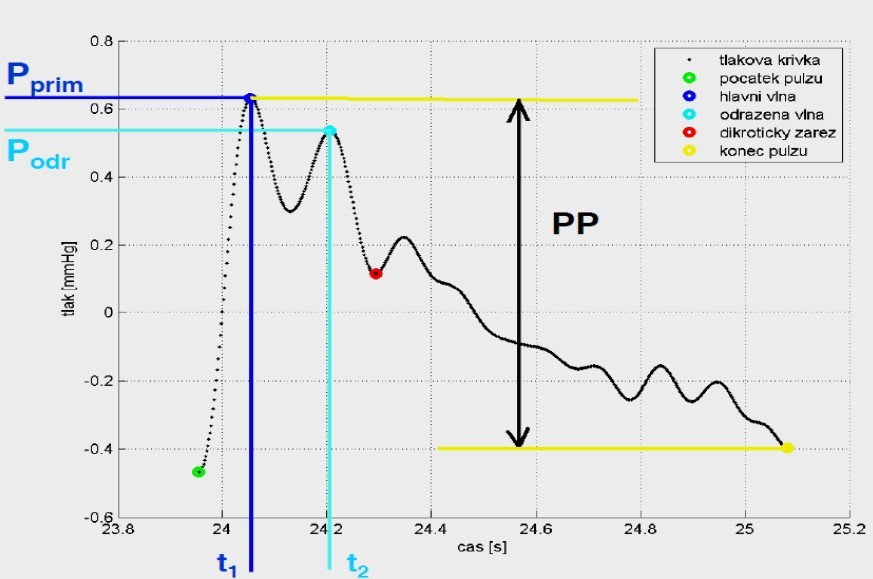
\includegraphics[width=1\textwidth]{pictures/pwv_pressure_wave.jpg}
\end{figure}
Kritéria pro PWV u člověka jsou
\begin{table}[H]
    \label{tab:pwv_criteria}
    \caption{Kritéria rychlosti pulzní vlny u člověka \cite{cite:Fabian}}
    \begin{ctucolortab}
        \begin{tabular}{ccc}
            \toprule
            PWV                & Jednotky      & Stav           \\ \midrule
            PWV < 7            &               & Optimální      \\
            7 $\leq$ PWV < 10  & $\frac{m}{s}$ & Normální       \\
            10 $\leq$ PWV < 12 &               & Zvýšené riziko \\
            12  $\leq$ PWV     &               & Abnormální     \\

            \bottomrule
        \end{tabular}
    \end{ctucolortab}
\end{table}
\section{Rešerše přístrojů pro měření hemodynamických parametrů krevního řečiště}
Tato sekce se zaměří na validované systémy na trhu pro neinvazivní měření hemodynamických parametrů krevního řečiště pomocí oscilometrické metody a to zejména na měření parametru PWV a analýzu pulzní tlakové křivky.

\subsection{SphygmoCor XCEL PWA/PWV}
SphygmoCor XCEL PWA/PWV je automatický systém pro analýzu krevní tlakové vlny pomocí pažní manžety.
\cite{cite:SphygmoCor}
\begin{figure}[H]
    \caption{SphygmoCor XCEL PWA/PWV \cite{cite:SphygmoCor}}
    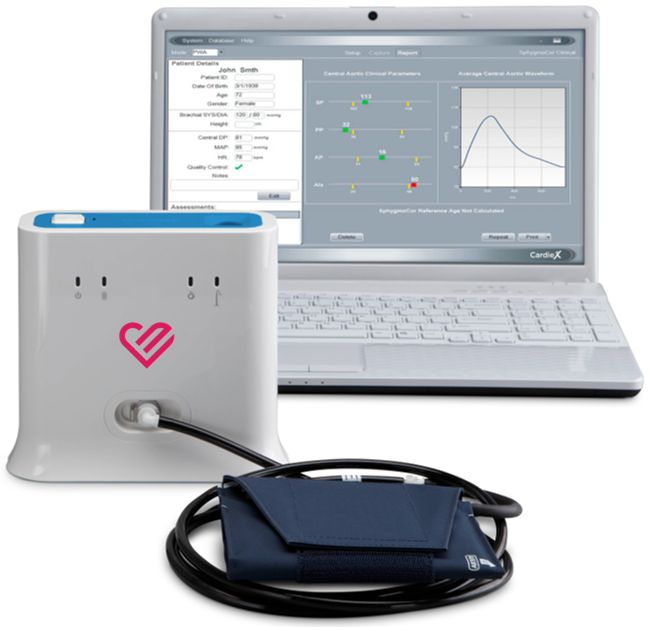
\includegraphics[width=0.8\textwidth]{pictures/XCEL_System.jpg}
\end{figure}
Mezi měřené parametry patří centrální aortální tlak, augmentační index a PWV. Pro měření parametru PWV je potřeba přidaná manžeta na stehno.
\cite{cite:SphygmoCor}
\par
Ovládání přístroje je pomocí připojeného osobního počítače přes USB s nainstalovaným softwarem. Software spouští terapii a následně dělá i vyhodnocení naměřených hodnot. Samostatný přístroj není schopný provádět terapii bez osobního počítače a dedikovaného softwaru.
\cite{cite:SphygmoCor}
\subsection{Uscom BP+}
Uscom BP+ je automatizovaný systém pro měření centrálního krevního tlaku, augmentačního indexu a analýzy křivky krevního tlaku a dalších parametrů při suprasystolickém tlaku.
Pro použití a operaci přístroje není za potřebí speciální školení uživatelům a najde uplatnění při hypertenzi, srdečním selhání, intenzivní péči a všeobecné praxi
\cite{cite:Uscom}
\begin{figure}[H]
    \caption{Uscom BP+ \cite{cite:Uscom}}
    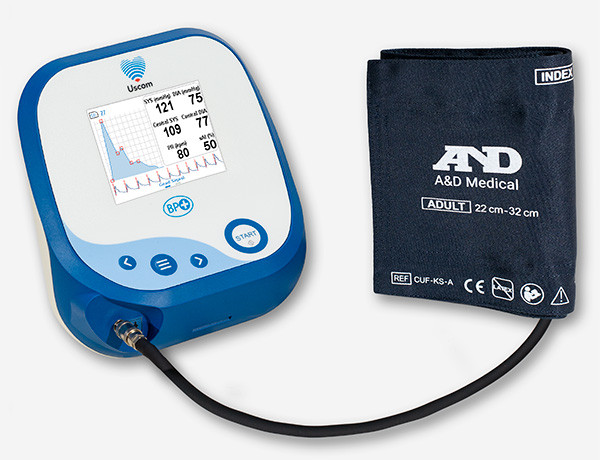
\includegraphics[width=0.8\textwidth]{pictures/uscom_bp.jpg}
\end{figure}
Systém BP+ provádí terapii a analýzu naměřených hodnot v jednom systému tj. bez potřeby nadřazeného systému.
\cite{cite:Uscom}
\subsection{Arteriograph}
Arteriograph (Tensiomed) je systém pro neinvazivní měření hemodynamických parametrů krevního řečistě oscilometrickou metodou a pomocí jedné pažní manžety.
Metoda měření oscilometrickou metodou je patentována (US Pat. No. 20070106162) a validována invazivně.
\begin{figure}[H]
    \caption{Tensiomed Arteriograph \cite{cite:Arteriograph}}
    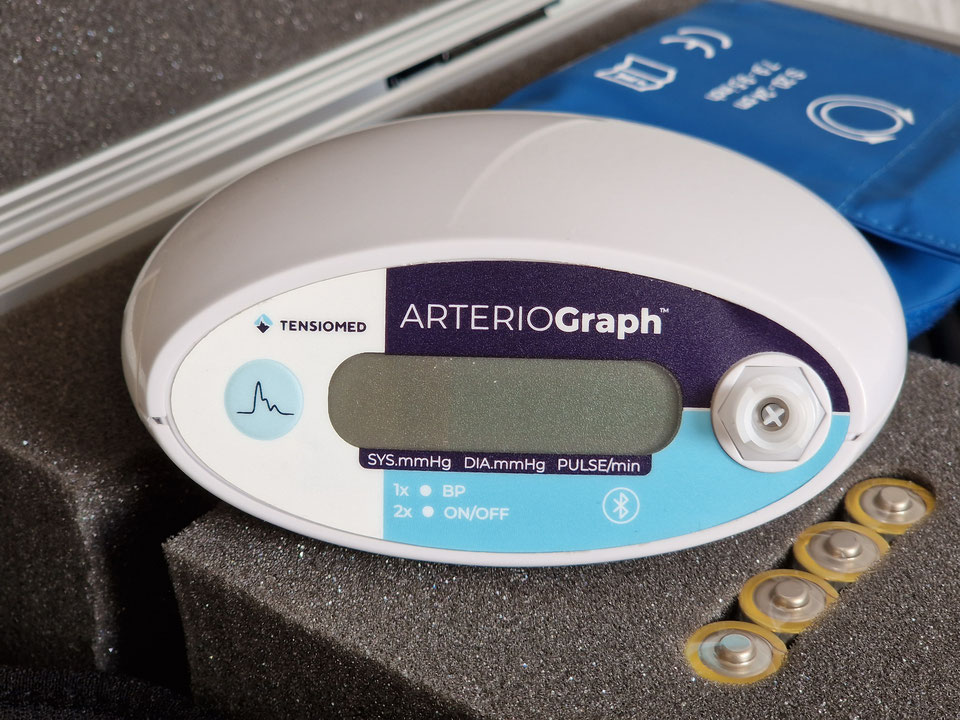
\includegraphics[width=0.8\textwidth]{pictures/arteriograph.jpg}
\end{figure}
Arteriograph může fungovat samostatně pro měření pouze krevního tlaku. Přístup k měření dalších hemodynamických parametrů je potřeba systém připojit k nadřazenému systému pomocí bluetooth s nainstalovaným specializovaným softwarem od Tensiomed.
Po připojení k nadřazenému systému, Arteriograph zasílá během terapie v reálném čase, kde se zpracují naměřené výsledky a zobrází.
\cite{cite:Arteriograph}

\subsection{Fukuda Denshi VaSera VS-1500N}
Diagnostický přístroj měřící stav cévního systému a provádějící screening aterosklerózy. Přístroj pracuje na principu měření pulsové vlny. Data jsou snímána ze čtyř tlakových manžet z končetin, dvou EKG elektrod a mikrofonu zaznamenávajícího srdeční ozvy.
Mezi měřené parametry patří srdeční frekvenci, tlak ve všech čtyřech končetinách, preejekční periodu, ejekční čas, čas dosažení maximálního tlaku a určuje biologický věk cév.\cite{cite:Vasera}
\begin{figure}[H]
    \caption{Fukuda Denshi VaSera VS-1500N \cite{cite:Vasera}}
    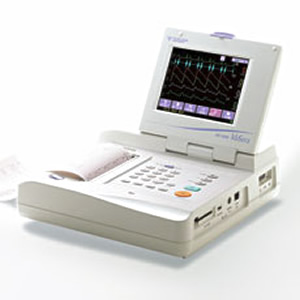
\includegraphics[width=0.8\textwidth]{pictures/vs_1500n.jpg}
\end{figure}
Mezi do počítávané parametry patří rychlost pulzní vlny, CAVI, ABI a další. Možnost měření PWV, EKG je možné, až po připojení volitelných modulů.\cite{cite:Vasera}
\par
Systém se dá použít samostatně bez nadřazeného systému, ale může se připojit pomocí softwaru VSS-10, který umožňuje archivaci, porovnávání a export dat. Umí ukládání pacientský dat na paměťovou kartu Compact Flash a uvnitř systému je
vestavěná barevná tiskárna zapisující na termopapír o šířce 145 mm.\cite{cite:Vasera}
